\documentclass{article}


% Meta data for this specific project
\newcommand{\projectName}{uFit}
\newcommand{\docTitle}{Detectação de Passos}
\date{}

% Create a new command to be used in the align environment in multiple line equations do only the last equation is numbered  
\newcommand{\n}{\nonumber \\ }

% Set the author and title of the document
\author{}
\title {\docTitle}



% Add all the basic packages 
\usepackage[margin = 1.25in, bottom = 60mm, top = 15mm]{geometry}
\usepackage{indentfirst}
\usepackage{fancyhdr}
\usepackage{tcolorbox}
\usepackage{graphicx}
\usepackage{amsmath}
\usepackage{hyperref}
\hypersetup{
    colorlinks=true,
    linkcolor=black,
    filecolor=magenta,
    urlcolor=cyan,
}



% Make the title centered both horizontally and vertically 
\usepackage{titling}
\renewcommand\maketitlehooka{\null\mbox{}\vfill}
\renewcommand\maketitlehookd{\vfill\null}


% Add the Mecatron Name on the left side of the page as background image
\usepackage[pages=all]{background}
\backgroundsetup{
scale=1,
color=black,
anchor=below,
position={-1,2.5},
opacity=1,
angle=0,
contents={%
  \includegraphics[height=150mm]{/Users/pedrocruz/Documents/LaTex/Mecatron/img/Mecatron_Side.png}
  }%
}


% Set the style for the cover page 
\fancypagestyle{documentCover}{

    %%%%%%%%%%%%%%%%%%%%%%%%%%%%%%%% Heading %%%%%%%%%%%%%%%%%%%%%%%%%%%%%%%%
    
    \setlength\headheight{80pt} %Enlarge the header space so we can add the logo
    \pagestyle{fancy}
    \fancyhf{}
    \renewcommand{\headrulewidth}{0pt} % Remove the horizontal header line
    \rhead{
        \includegraphics[width = 40mm]{/Users/pedrocruz/Documents/LaTex/Mecatron/img/Screen Shot 2020-08-15 at 7.51.37 PM.png}
    }
    
}

% Set the page style to use fancy header for the body of the document 
\fancypagestyle{documentBody}{

    %%%%%%%%%%%%%%%%%%%%%%%%%%%%%%%% Heading %%%%%%%%%%%%%%%%%%%%%%%%%%%%%%%%

    \setlength\headheight{100pt} %Enlarge the header space so we can add the logo
    \pagestyle{fancy}
    \fancyhf{}
    \renewcommand{\headrulewidth}{0pt} % Remove the horizontal header line
    \rhead{
        \includegraphics[width = 40mm]{/Users/pedrocruz/Documents/LaTex/Mecatron/img/Screen Shot 2020-08-15 at 7.51.37 PM.png}
    }
    
    %%%%%%%%%%%%%%%%%%%%%%%%%%%%%%%% Footing %%%%%%%%%%%%%%%%%%%%%%%%%%%%%%%%

    \fancyfoot[C]{
        \includegraphics[width = 150mm]{/Users/pedrocruz/Documents/LaTex/Mecatron/img/Horizontal_Bar.png} \\ 
        Mecatron Projetos e Consultoria Júnior - UNICAMP \\ 
        \projectName 
        \begin{flushright}
            \thepage
        \end{flushright}
    }

    
}


\begin{document}
    
    \maketitle
    \thispagestyle{documentCover}
    
  
    \newpage
    \pagestyle{documentBody}
    \tableofcontents
    \newpage

    \section{Sensor}
        Para captarmos quando que o usuário dá um passo estaremos utilizando o sensor MPU6050, o qual apresenta um
        giroscópio e um acelerômetro embutidos. 
    
        \subsection*{Acelerômetro}
            Para nossa aplicação de deteção de passos utilizaremos somente as capacidades de acelerômetro do
            MPU6050.
            Um acelerômetro é capaz de determinar a aceleração gravitacional linear sofrida por um corpo em todas as 3
            dimensões $(x,y,z)$. Como o usuário estará sempre na vertical a componente $G_z$ (componente da
            aceleração gravitacional no eixo $z$) terá variação mínima e insignificante para a detectação dos
            passos dados pelo usuário. Com isso temos a seguinte representação gráfica dos dados captados pelo
            MPU6050: 
            
            \begin{figure}[h!]
                \centering
                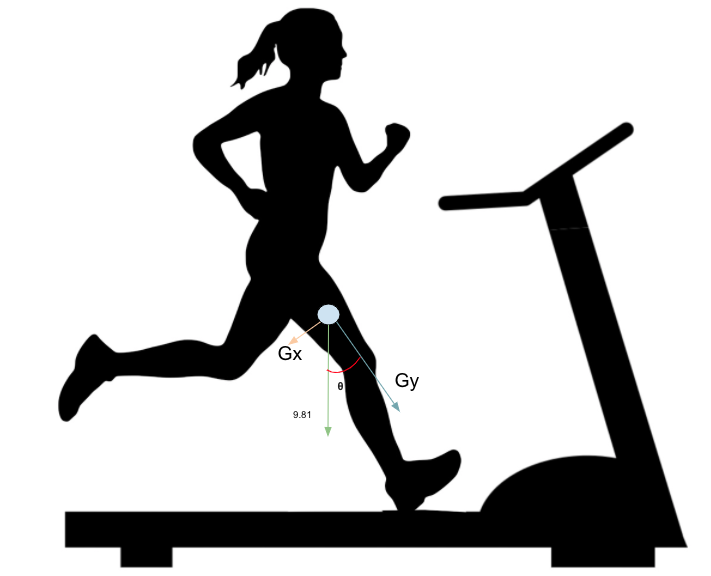
\includegraphics[width=.7\textwidth]{img/Screen Shot 2020-10-06 at 8.17.44 PM.png}
            \end{figure}
        
   
            A partir dos dados presentes na imagem acima, sendo $G_y$ e $G_x$ os valores de aceleração
            retornados pelo acelerômetro, nós somos capazes de calcular o ângulo $\theta$ pela utilização da
             relação trigonométrica \ref{eq:arccos_theta}:

            \begin{align}
                \cos{\theta} = \frac{G_y}{9.81} \n 
                \theta = \arccos{\frac{G_y}{9.81}} \label{eq:arccos_theta}
            \end{align}

            Tendo o valor de $\theta$ e tendo a altura do usuário seremos capaz de determinarmos a distância
            percorrida pelo usuário pela meia passada dada. Com isso conseguimos somar duas meia passadas
            seguidas e achar o $\Delta S$ de cada passo que o usuário dá.

        \section{Processamento de Sinal}
            O sensor MPU6050 é extremamente sensível (como demonstra a imagem \ref{img:raw_plot}) o que se demonstra algo
            prejudicial para a aplicação em questão, pois resulta na contagem de falsos passos no cenário de
            possíveis choques mecânicos. A fim de evitar a ocorrência desses outliers serem contados como
            passos, será utilizado um método de \textit{signal smoothing} chamado de ``Gaussian Moving Average /
            Gaussian Filter", que consiste de uma média ponderada móvel de 100 data points, tendo os valores
            de uma distribuição Gaussiana Normal como os pesos para a média. A vantagem desse método de
            processamento de sinal é sua relativa rapidez na velocidade de computação e, principalmente, o
            fato de que mantém as tendências do data set original. Implicando que podemos usar a derivação e
            outras ferramentas matemáticas sem que haja uma perda significativa na hora de sua interpretação.
            
            \begin{figure}[h!]
                \centering
                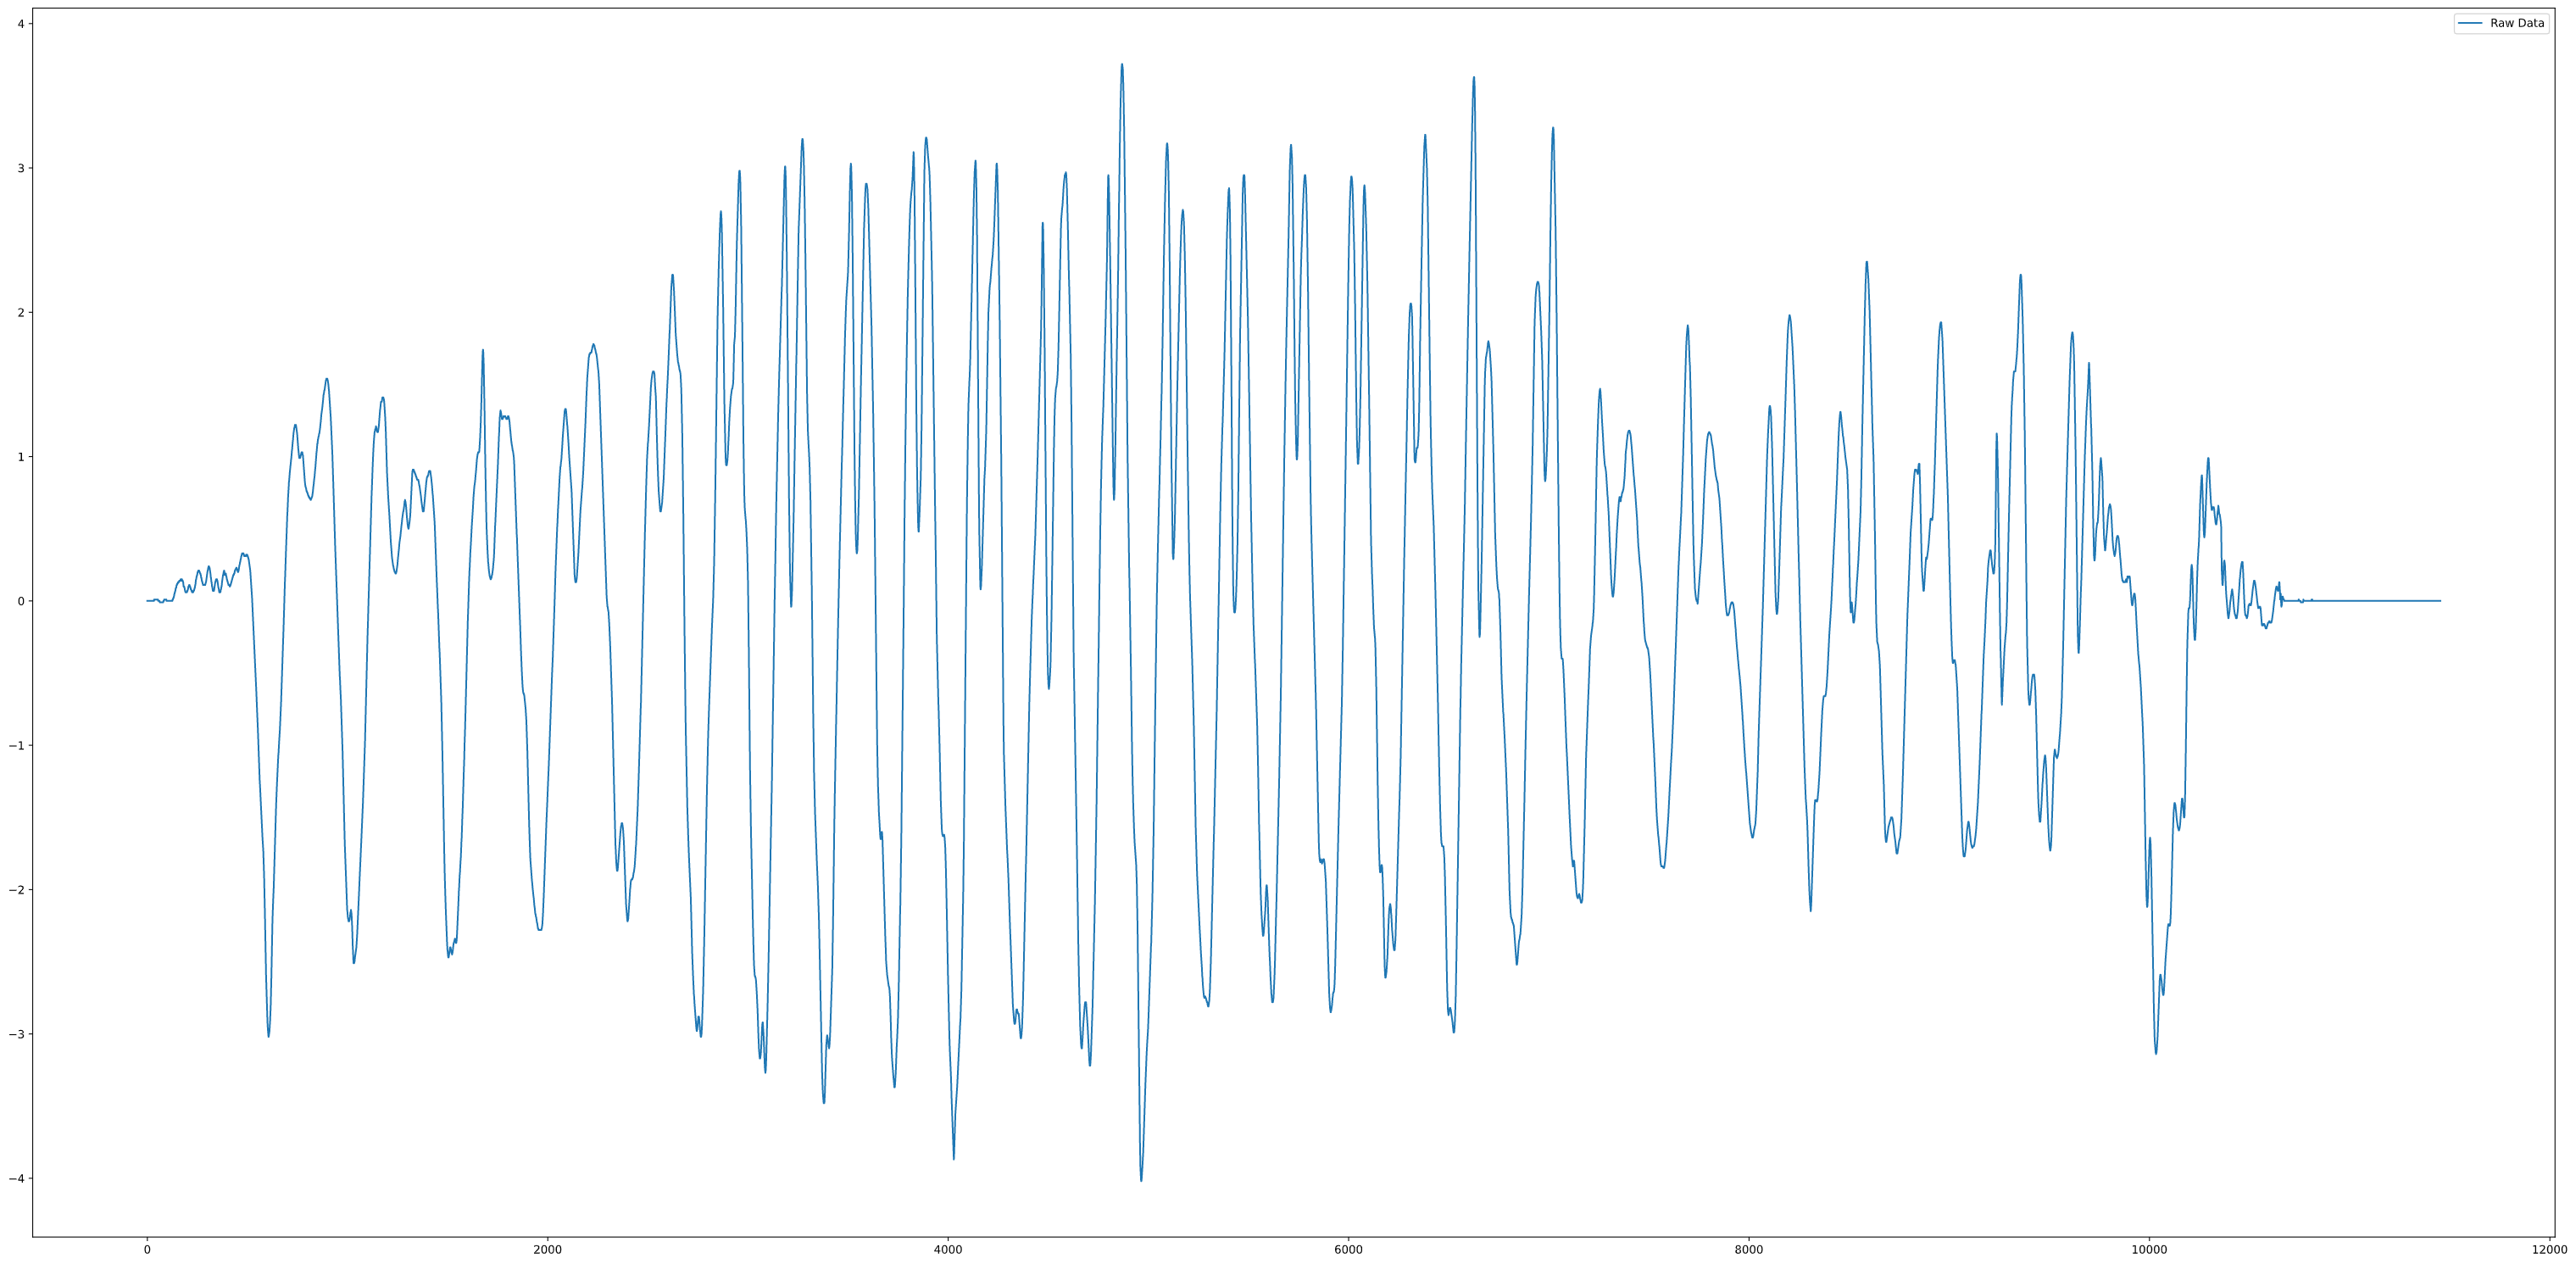
\includegraphics[width=.8\textwidth]{img/Raw_Data.png} 
                \caption{Gráfico $G_x \times t(s)$ sem correção de sinal}
                \label{img:raw_plot} 
            \end{figure}

            \begin{figure}[h!]
                \centering
                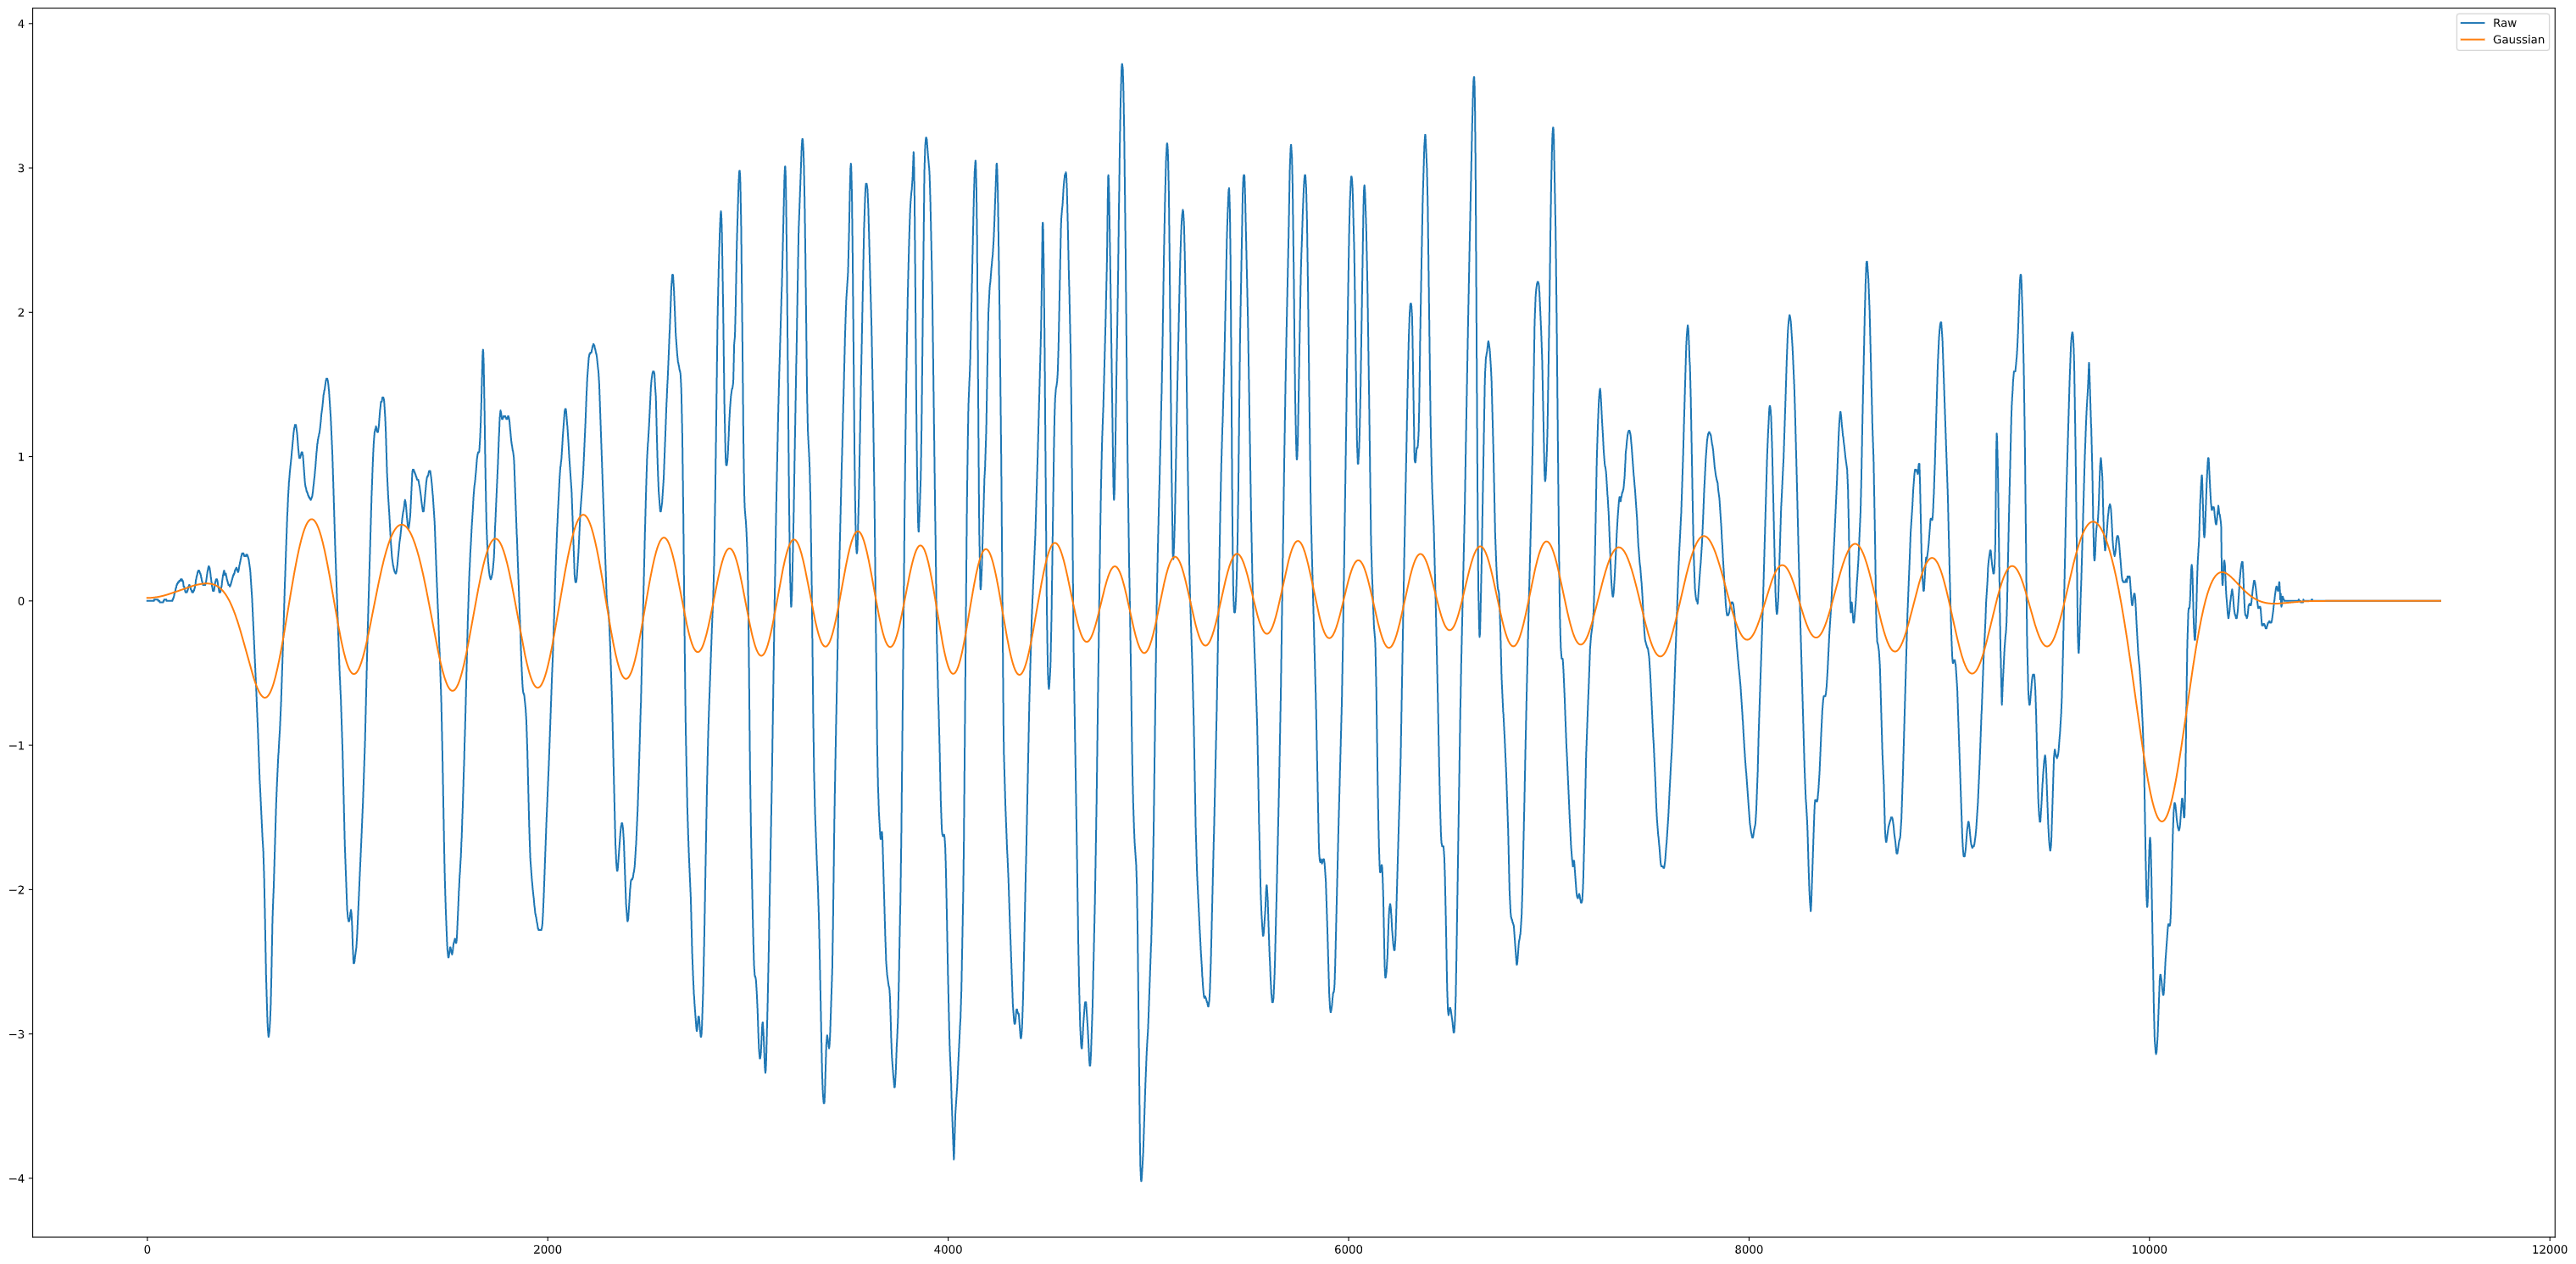
\includegraphics[width=.8\textwidth]{img/Smoothed_data.png}
                \caption{Gráfico $G_x \times t(s)$ com correção de sinal (em laranja)}
                \label{img:smoothed_plot} 
            \end{figure}

        \section{Deteção de Passos}
        Fazendo o estudo do comportamento dos valores de $G_x$ retornados pelo acelerômetro vemos que, assim
        que o usuário está com sua perna na posição mais esticada (assim que ocorre o contato entre o
        calcanhar com o chão) ,temos que a componente $G_x$  assume seu valor máximo. Tendo isso em mente,
        precisamos somente identificar quando $G_x$ é um máximo local, computar um passo dado, utilizar a
        equação \ref{eq:arccos_theta} para calcular o ângulo $\theta$ e, por conseguinte, $\Delta S$ da
        passada.

        Para detectarmos se $G_x$ é um máximo local podemos simplesmente calcularmos a derivada $G_x'$. A
        derivada nada mais é do que a inclinação da reta tangente a um ponto de uma função (no caso da função $G_x'(t)$).
        Quando a função $G_x$ está no seu ponto máximo, a inclinação da reta tangente é igual a zero, em
        outras palávras:

        \begin{align}
            G_x(t) = G_{x_{Max}} \iff G_x'(t) = 0
        \end{align}
\end{document}